\subsection{Bubble \& eat} \label{bubbleeat}

\subsubsection{Package}
Il package della demo Bubble \& eat è composto da due ulteriori packages: \Customer{}\footnote{Per uniformare quanto presentato nell'\AnalisiDeiRequisiti{} con il prodotto finale, il linguaggio utilizzato per la nomenclatura è l'inglese. Sono stati dunque tradotti gli attori individuati nel corrispettivo termine inglese.} e \textit{Restaurant}. 
Il primo si riferisce soltanto all'utente \Customer{}. Il secondo invece contiene i package di tutti gli altri attori:
\begin{itemize}
	\item \Manager{};
	\item \Chef{};
	\item \Deliveryman{};
	\item \Purchasingmanager{}.
\end{itemize}
Nel package Restaurant, inoltre, è anche contenuto il pacchetto Order\-Gateway.\\
Lo scopo del package Order\-Gateway è quello di creare, modificare ed eliminare le ordinazioni interagendo con il database che le contiene.
Tutti gli attori interni ed esterni al ristorante hanno dipendenze verso l'Order\-Gateway.
\begin{figure}[H]
	\centering
	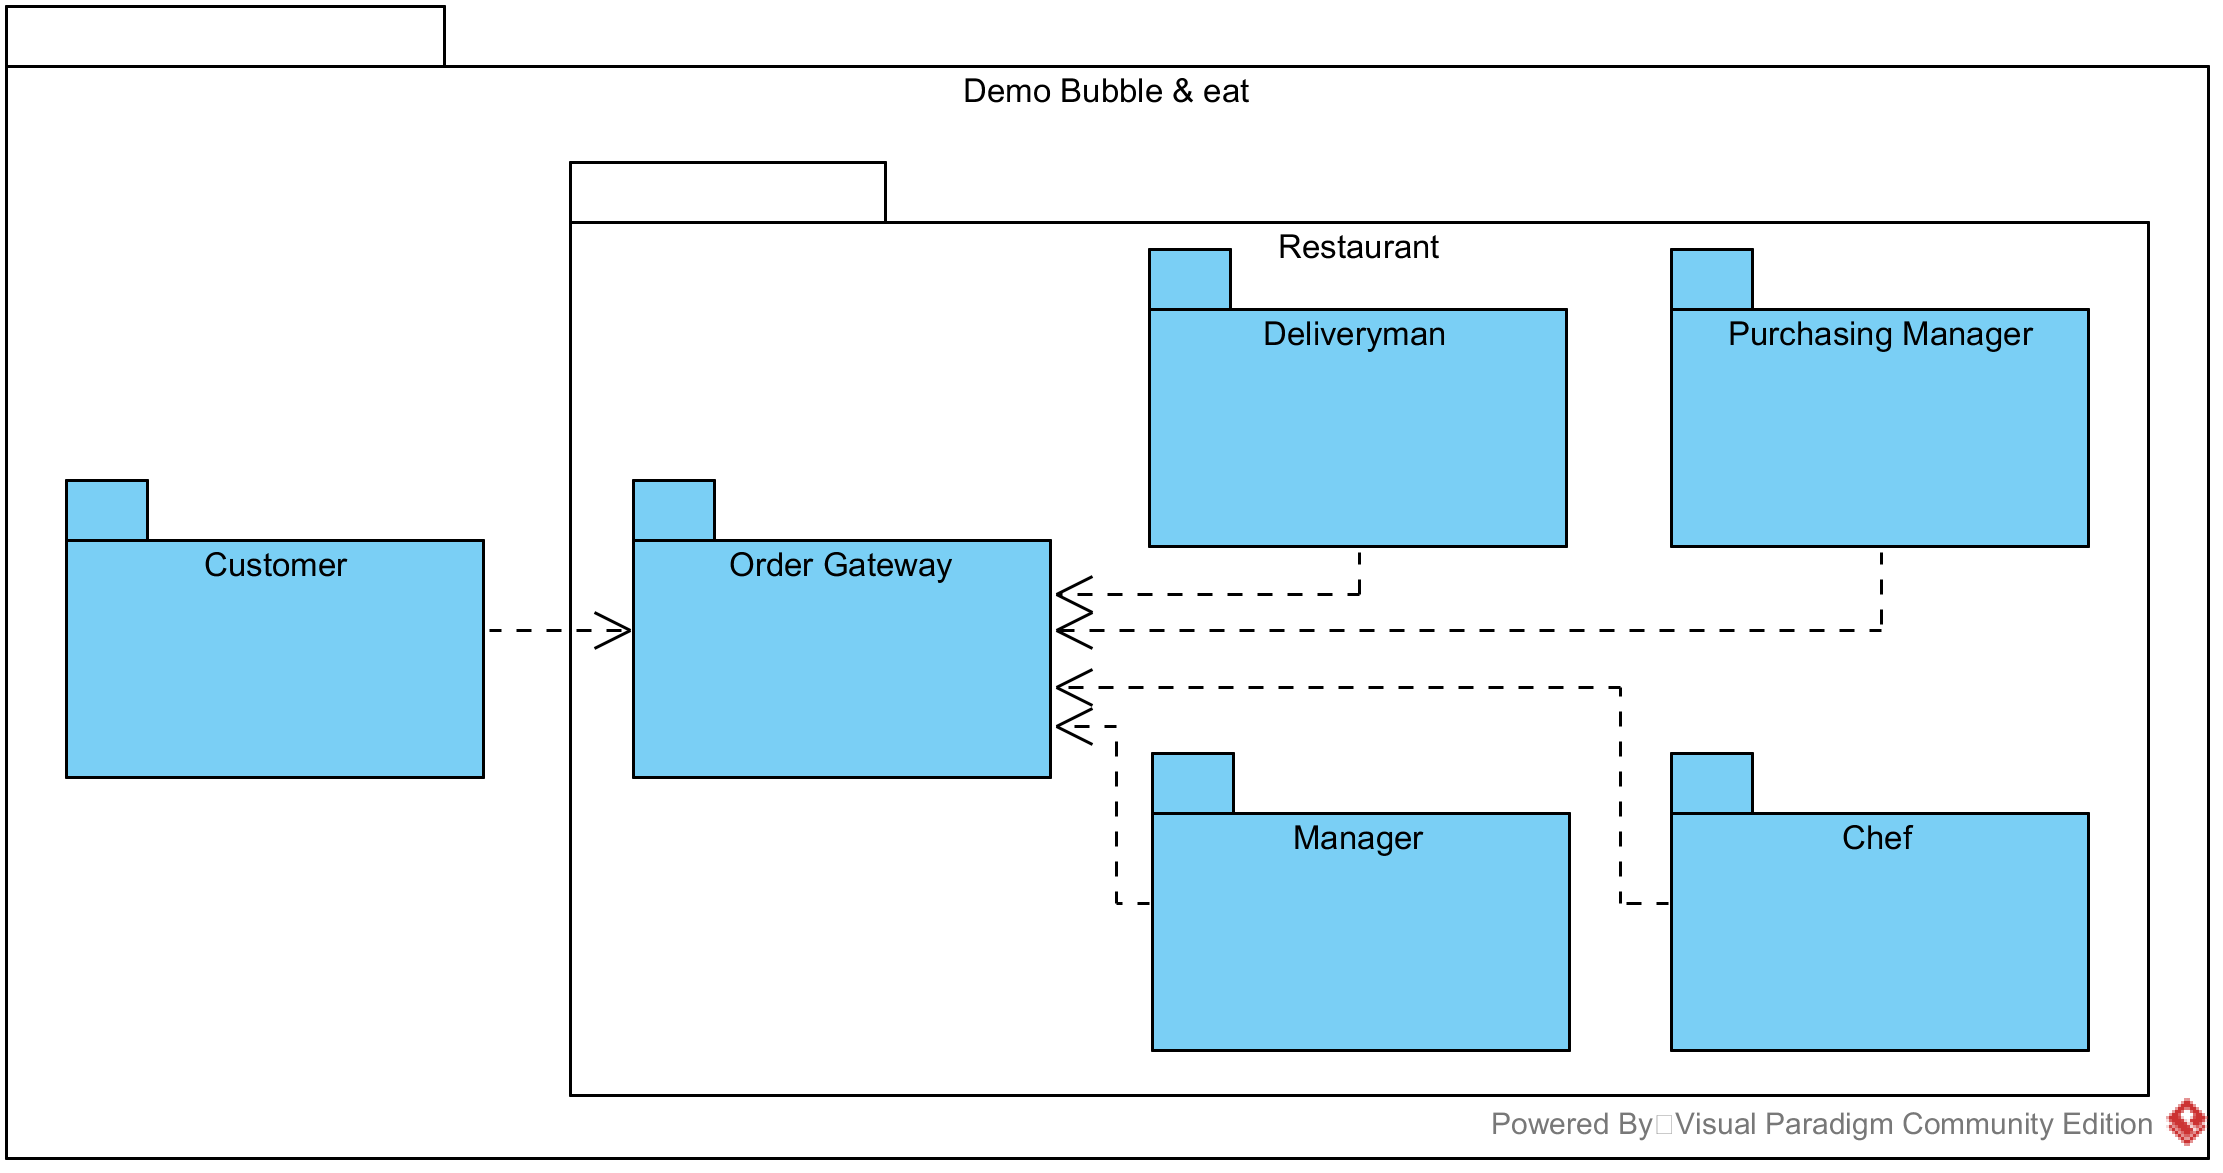
\includegraphics[width=14cm]{diagrammi_img/classi_e_package/demo_packages.png}
	\caption{Demo Bubble \& eat}
\end{figure}

\subsubsection{Package Order\-Gateway OLD}
Il package Order\-Gateway si occupa di gestire le interazioni tra attori e database e le eventuali comunicazioni tra gli attori stessi. Il package internamente è composto dalle classi Order\-Gateway e Menu e dal package Orders.\\
Il package Orders definisce le ordinazioni e la collezione di queste ultime che verranno poi costruite seguendo il Factory method come design pattern dalla classe Menu.\\
Tutte le interazioni con gli elementi descritti sopra sono rese disponibili agli attori dalla classe Order\-Gateway.
\begin{figure}[H]
	\centering
	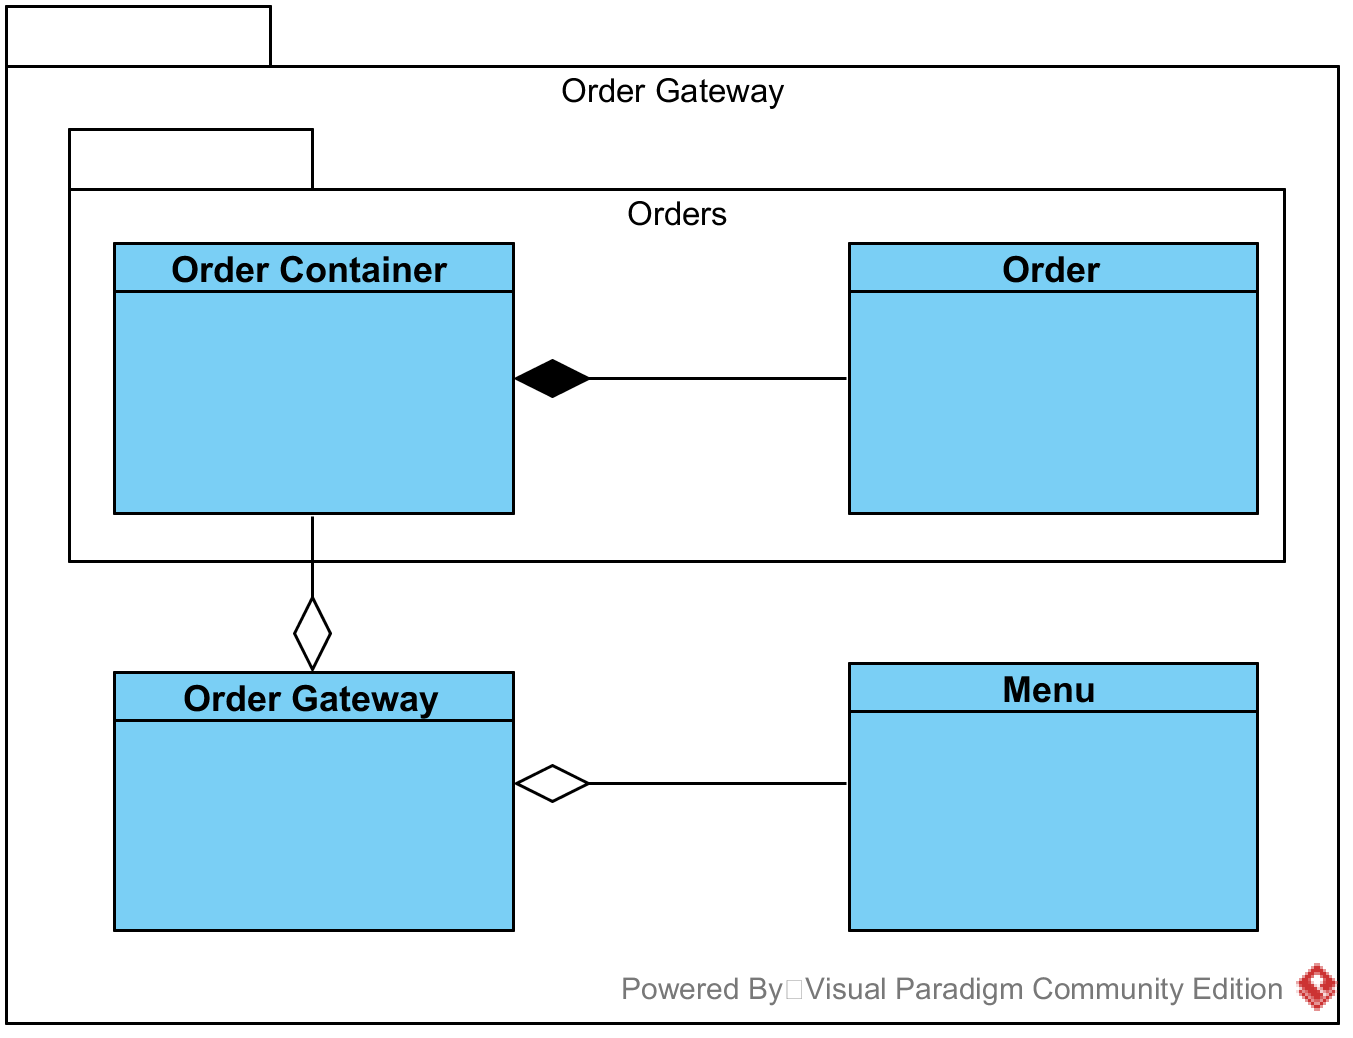
\includegraphics[width=14cm]{diagrammi_img/classi_e_package/ordergate.png}
	\caption{Package Order\-Gateway}
\end{figure}

\subsubsection{Package Order\-Gateway NEW}
Il package Order\-Gateway si occupa di gestire le interazioni tra attori e database e le eventuali comunicazioni tra gli attori stessi. Il package internamente è composto dalle classi Order\-Gateway ed i package Handlers, States, Reducer, Action e Server.\\
La classe order\-gateway si occupa di indirizzare le diverse utenze all'handler corretto e gestisce la connessione con il database e le ordinazioni.\\
Il package Handlers contiene la classi dedicate alla gestione delle diverse tipologie di utenza.\\
Il package States contiene le classi che si occupano a salvare lo stato dei componenti.\\
Il package Reducer contiene le classi che che interagiscono con il package States per aggiornare gli stati dei componenti.\\
Il package Action contiene le classi che si occupano della gestione delle funzionalità dell'Order\-Gateway.\\
Il package Server contiene la classe server e si occupa di istanziarla e di gestire i socket.\\
\begin{figure}[H]
	\centering
	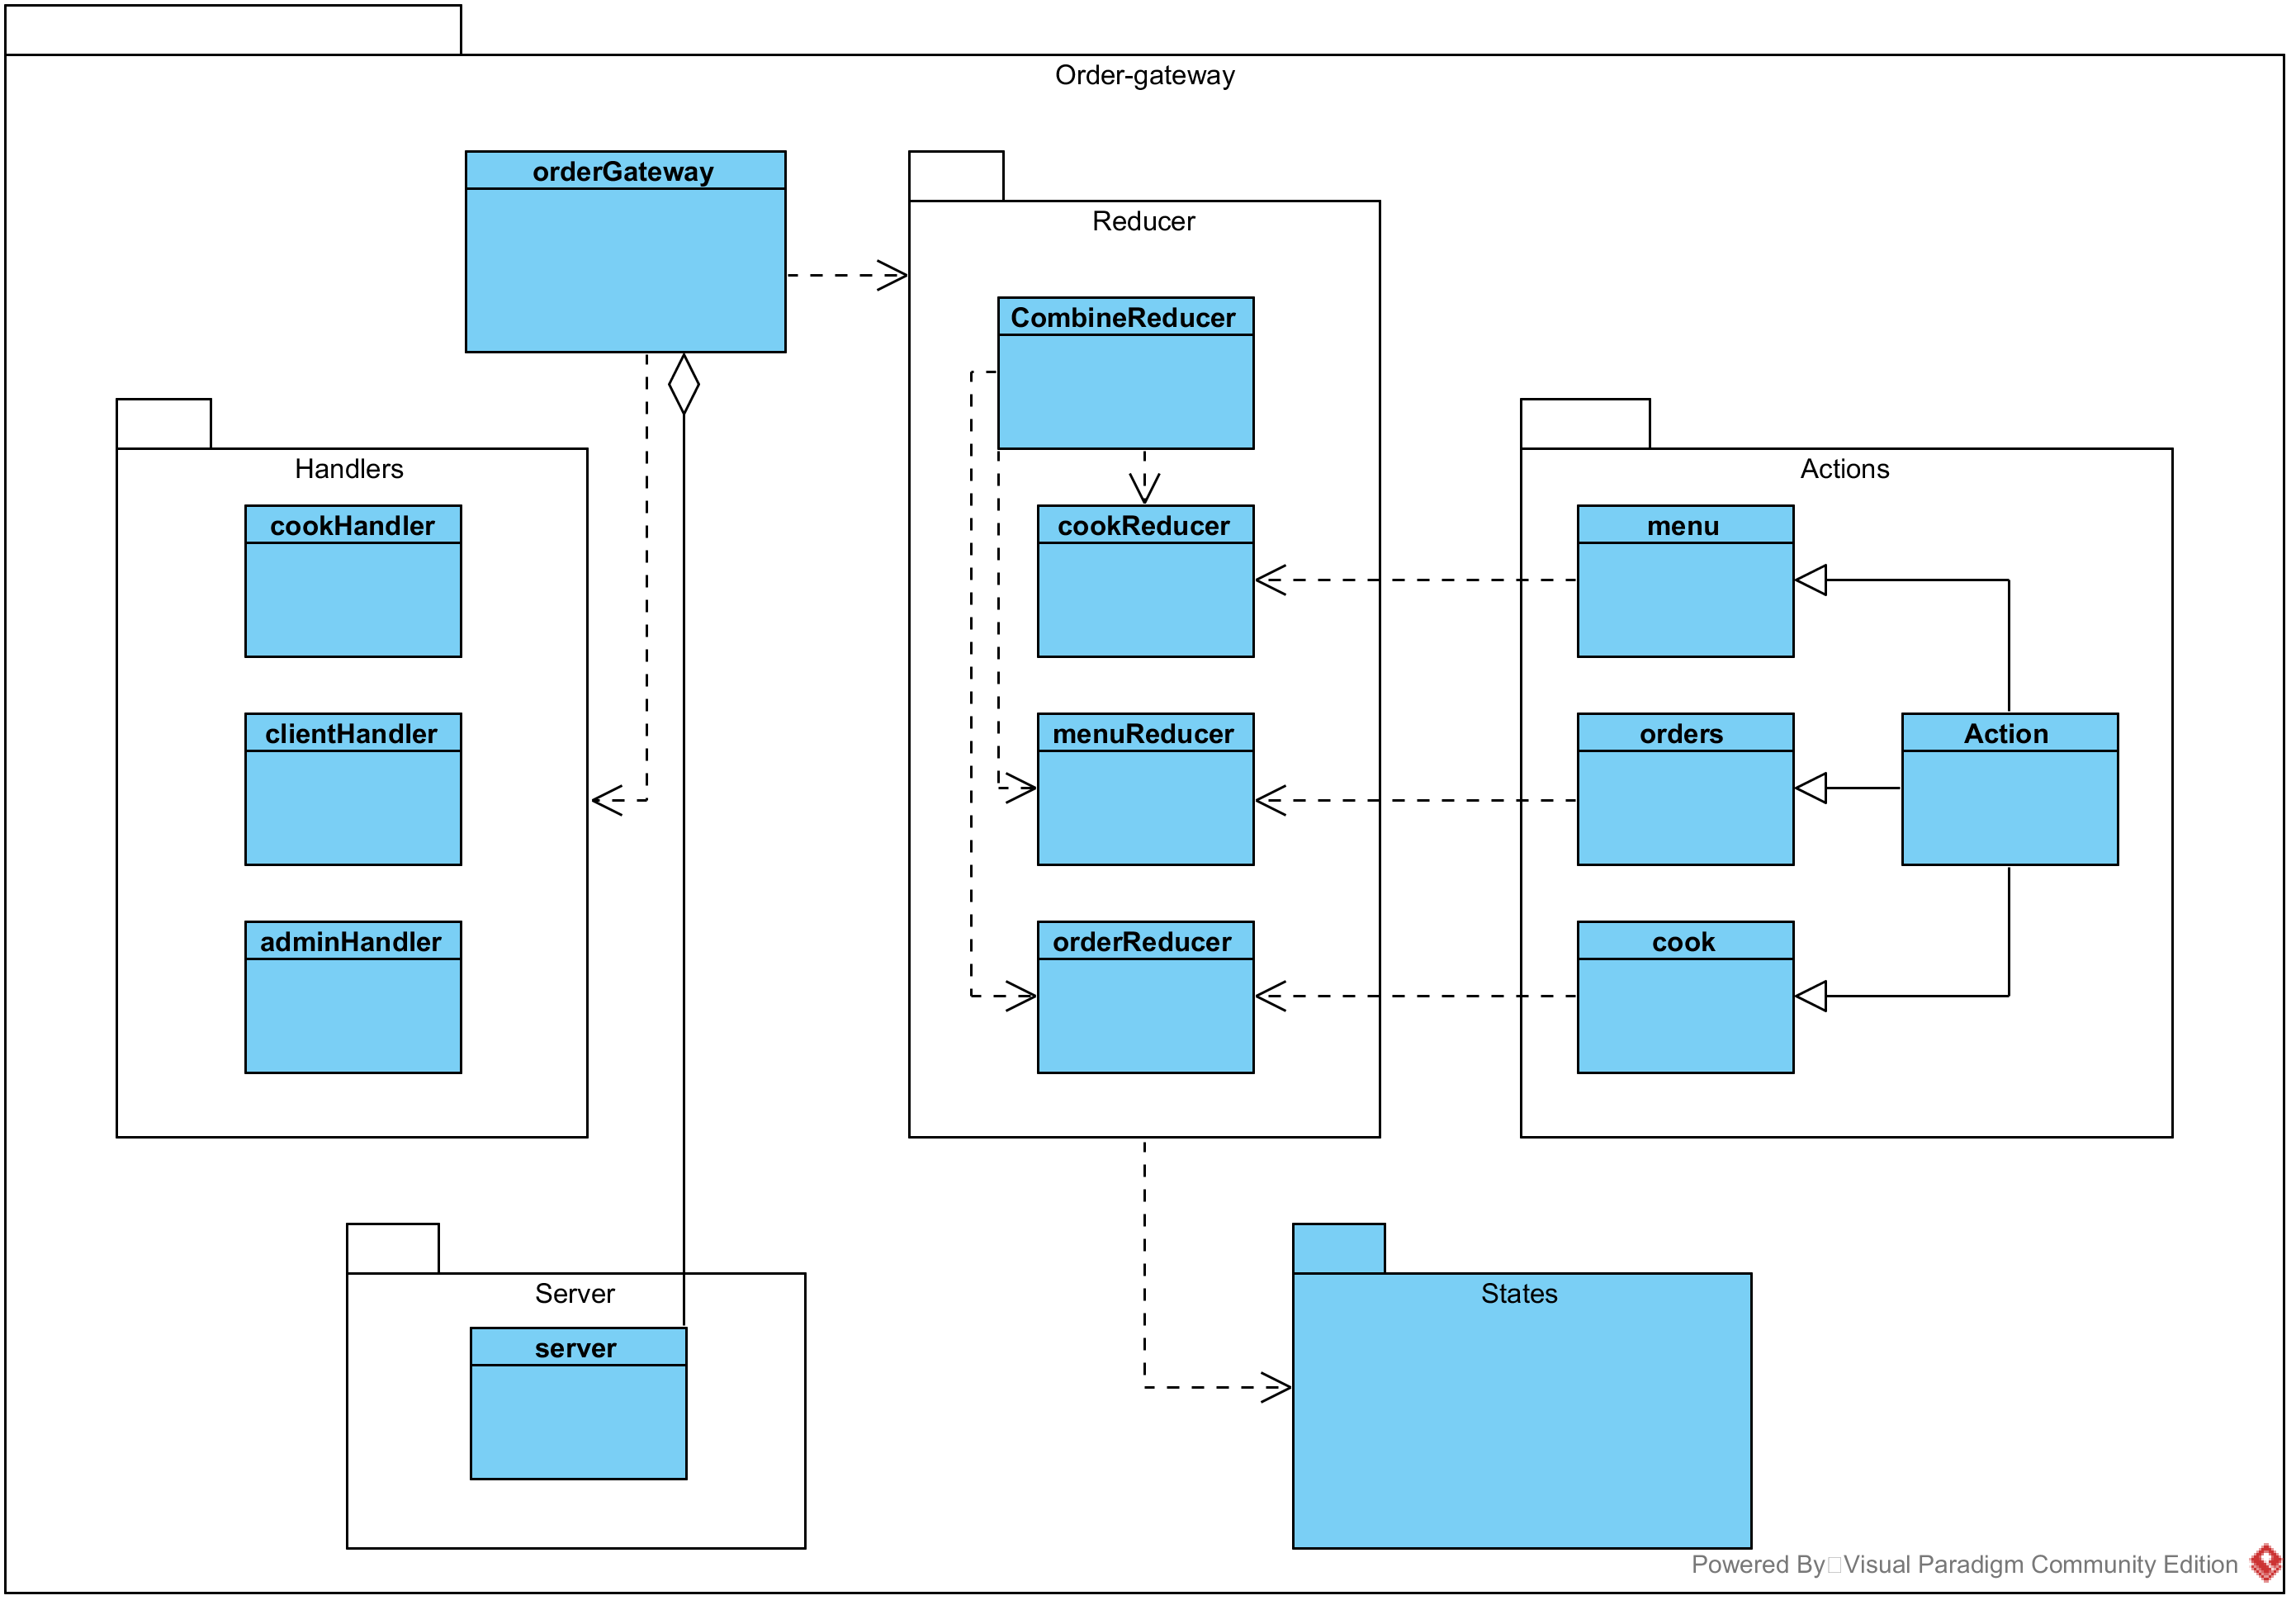
\includegraphics[width=14cm]{diagrammi_img/classi_e_package/ordergateNEW.png}
	\caption{Package Order\-Gateway}
\end{figure}

\subsubsection{Struttura delle classi}
La Demo Bubble \& eat può essere divisa in due categorie di classi principali:
\begin{itemize}
	\item gli attori, a loro volta divisi in interni, quali \Manager{}, \Chef{}, \Deliveryman{} e \Purchasingmanager{}, ed un unico attore esterno, il \Customer{};
	\item un Hub gestionale centrale, l’Order\-Gateway.
\end{itemize}
Le classi degli attori non avranno la possibilità di manipolare direttamente il database o comunicare tra loro ma potranno farlo attraverso alla classe Order\-Gateway.
I singoli attori avranno la possibilità di manipolare e visualizzare gli stessi dati in modi differenti determinati dalla loro tipologia di utenza.
Tutte le operazioni saranno fornite dall'Order\-Gateway che si occuperà, oltre che dell'interazione con il database, anche della creazione degli Order.

\begin{figure}[H]
	\centering
	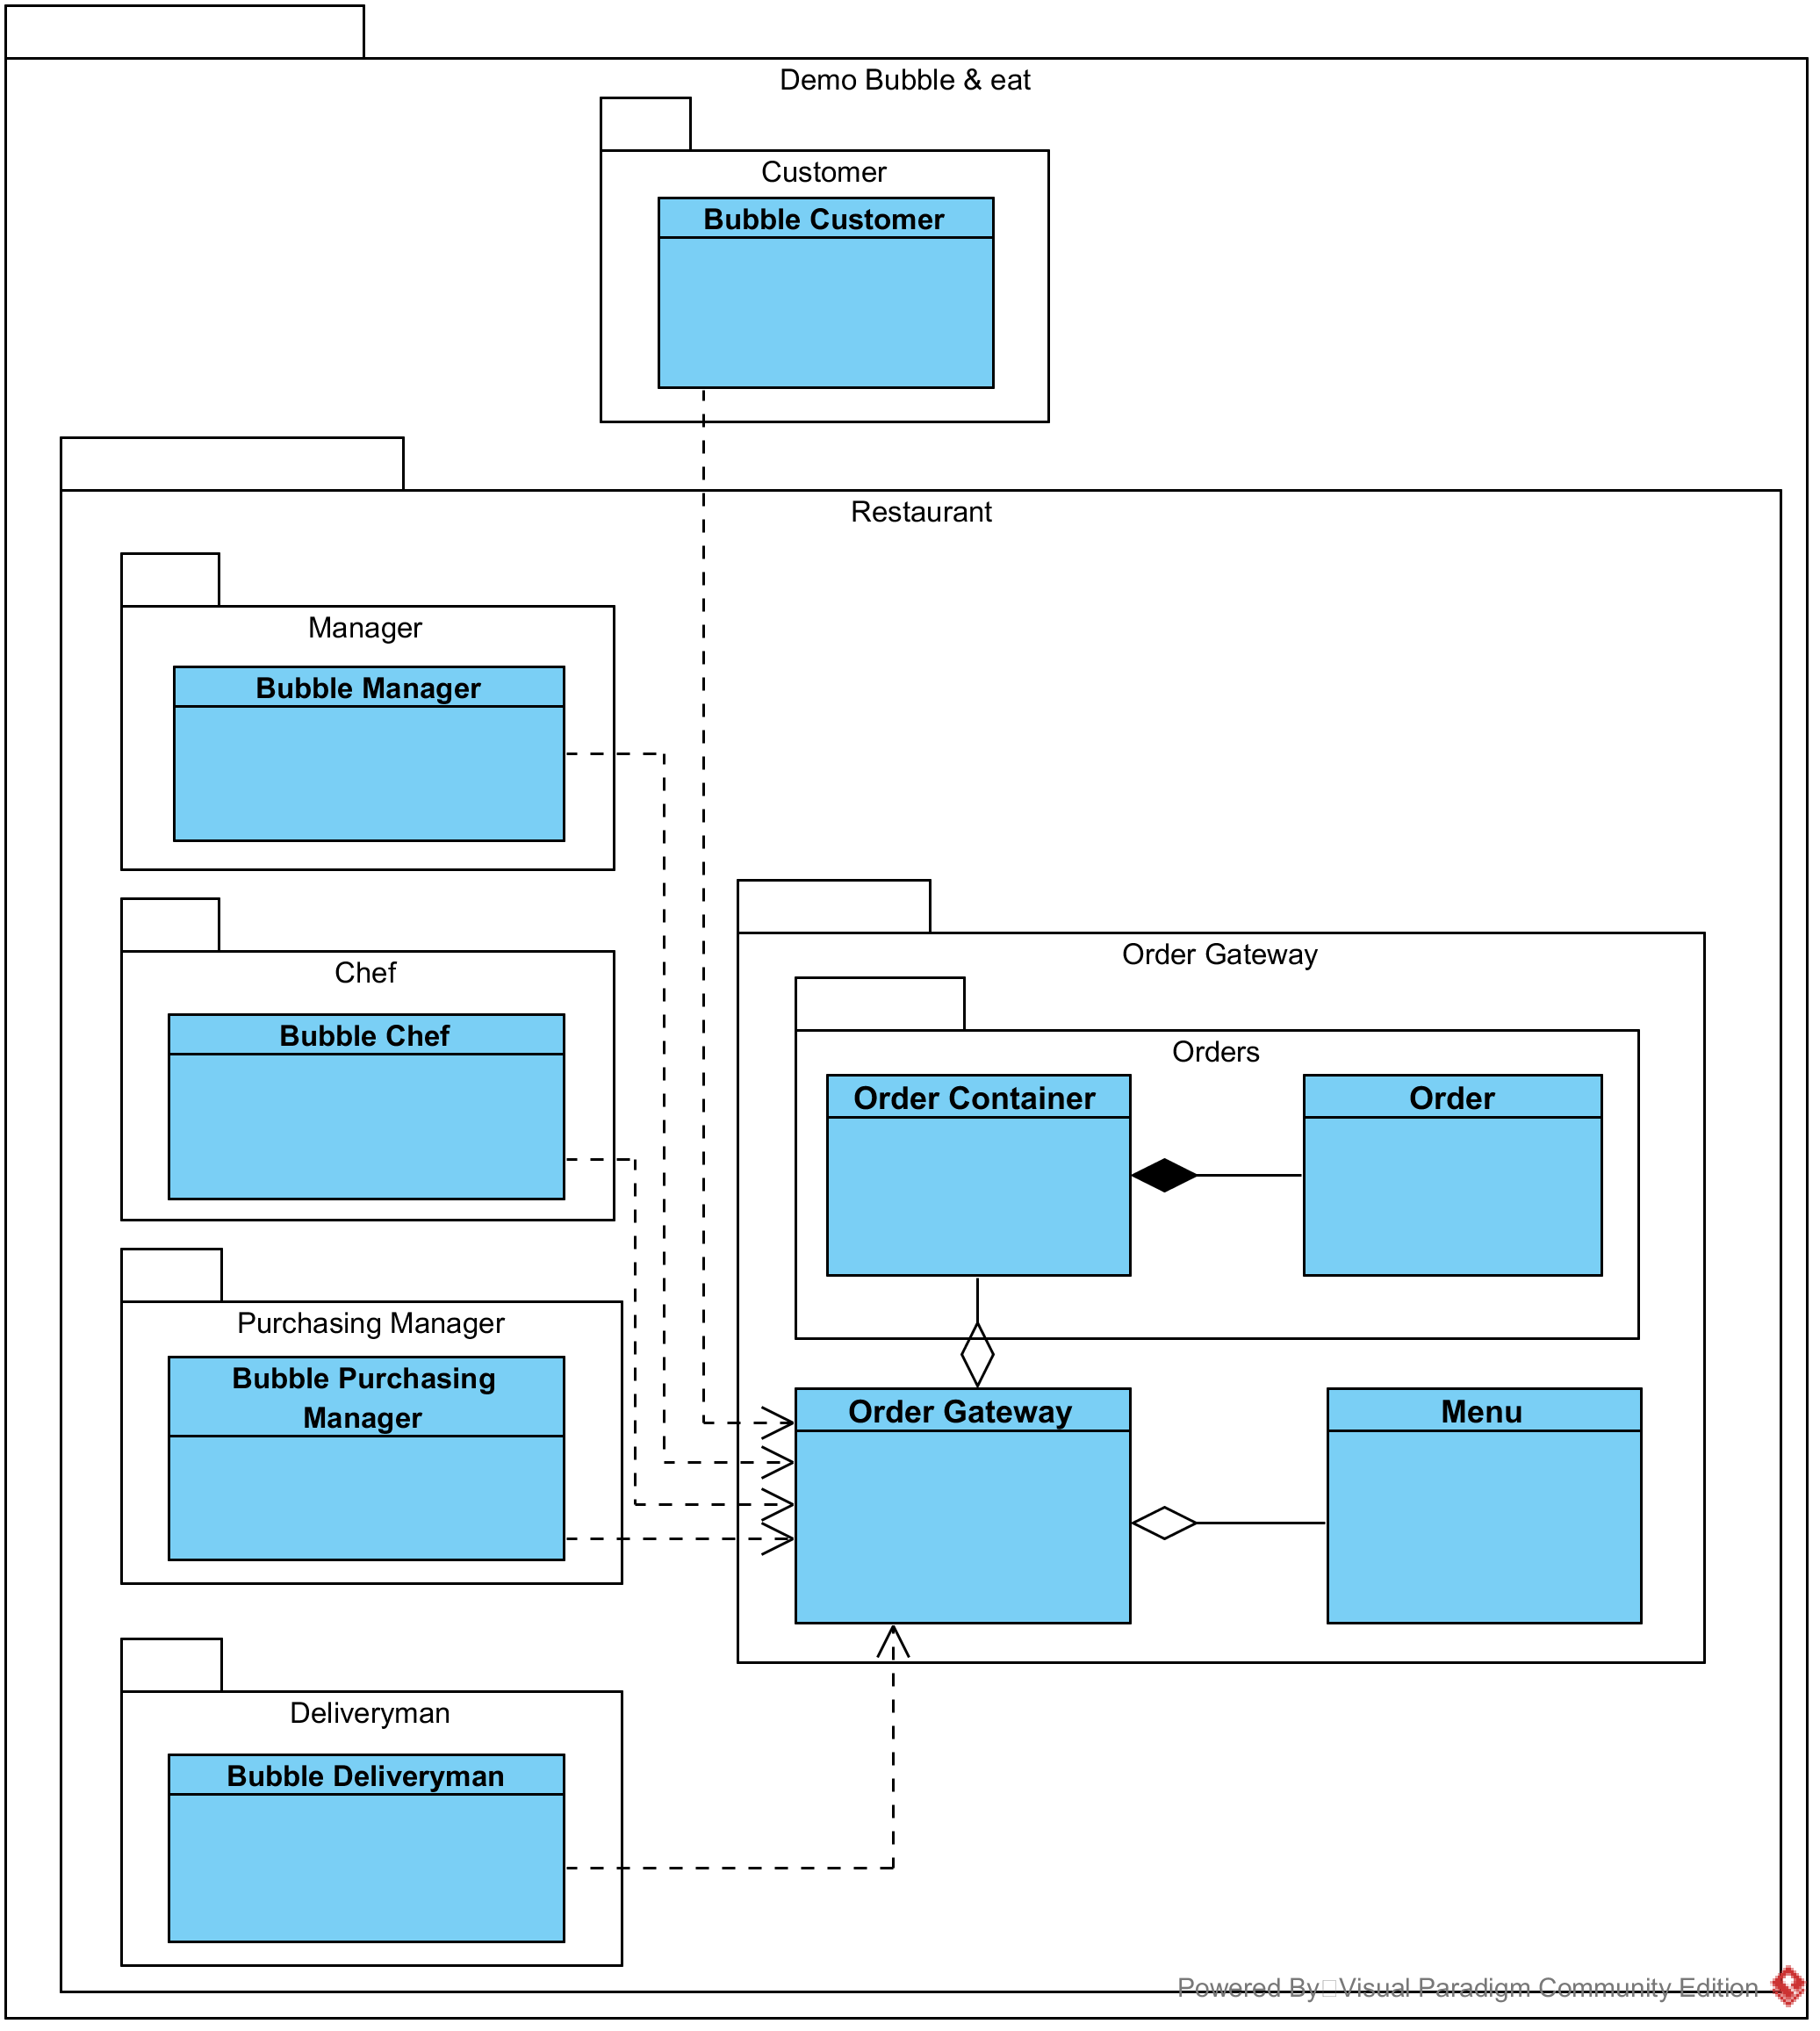
\includegraphics[width=13cm]{diagrammi_img/classi_e_package/demo_classes.png}
	\caption{Diagramma di struttura delle classi}
\end{figure}

\subsubsection{Descrizione classi}

\paragraph{DemoBubble\&eat\-::Customer\-::Bubble\-Customer}\label{eat-customer}\mbox{}\\
\textbf{Descrizione:}\\
La classe permette al \Customer{} di consultare il menu, registrare i propri dati personali e inviare le proprie ordinazioni.\\
\textbf{Utilizzo:}\\
Questa classe attraverso l'Order\-Gateway riceve il menu da consultare per mezzo del quale può creare la propria ordinazione.

\paragraph{Demo\-Bubble\&eat\-::Restaurant\-::Manager\-::Bubble\-Manager}\label{eat-manager}\mbox{}\\
\textbf{Descrizione:}\\
La classe permette al \Manager{} di gestire il menu, il magazzino e le ordinazioni.\\
\textbf{Utilizzo:}\\
Questa classe permette di gestire tutte le operazioni fornite da Order\-Gateway ed ha la possibilità di manipolare il magazzino e le ordinazioni.

\paragraph{Demo\-Bubble\&eat\-::Restaurant\-::Chef\-::Bubble\-Chef}\label{eat-chef}\mbox{}\\
\textbf{Descrizione:}\\
La classe permette allo \Chef{} di consultare le ordinazioni e di impostare lo stato di una ordinazione in modo da renderla disponibile alla consegna.\\
\textbf{Utilizzo:}\\
Questa classe, attraverso l'Order\-Gateway, recupera e visualizza le ordinazioni e offre la possibilità allo \Chef{} di modificarne lo stato.

\paragraph{Demo\-Bubble\&eat\-::Restaurant\-::Deliveryman\-::Bubble\-Deliveryman}\label{eat-deliveryman}\mbox{}\\
\textbf{Descrizione:}\\
La classe permette al \Deliveryman{} di consultare gli ordini pronti alla consegna, di ottenere i dati personali dei \Customer[2]{} relativi alle consegne selezionate e di eliminarle una volta completate.\\
\textbf{Utilizzo:}\\
Questa classe, attraverso l'Order\-Gateway, riceve la lista delle ordinazioni da consegnare, le visualizza e permette di selezionare le consegne ed eliminarle una volta selezionate.

\paragraph{Demo\-Bubble\&eat\-::Restaurant\-::PurchasingManager\-::Bubble\-Purcha\-sing\-Ma\-nager}\label{eat-purchasing}\mbox{}\\
\textbf{Descrizione:}\\
La classe permette al \Purchasingmanager{} di recuperare e visualizzare la lista della fornitura da acquistare oltre ad eliminare gli acquisti dalla lista.\\
\textbf{Utilizzo:}\\
Questa classe recupera dall'Order\-Gateway la lista degli acquisti, la visualizza e consente di eliminare gli acquisti presenti nella stessa.

\paragraph{Demo\-Bubble\&eat\-::Restaurant\-::Order\-Gateway\-::Order\-Gateway}\label{eat-gateway}\mbox{}\\
\textbf{Descrizione:}\\
La classe permette a tutti gli attori di interagire con il database e di effettuare la connessione con quest'ultimo. Inoltre si occupa di indirizzare gli utenti verso il proprio specifico handler.\\
\textbf{Utilizzo:}\\
La classe gestisce:
\begin{itemize}
	\item La connessione con il database ed il salvataggio dei dati;
	\item L'indirizzamento dei diversi utenti verso l'apposito Handler.\\
\end{itemize}
\textbf{Relazioni con altre classi:}\\
\begin{itemize}
	\item {Demo\-Bubble\&eat\-::Restaurant\-::Order\-Gateway\-::Server\-::Server};
	\item {Demo\-Bubble\&eat\-::Restaurant\-::Order\-Gateway\-::Handlers\-::Cook\-Handler};
	\item {Demo\-Bubble\&eat\-::Restaurant\-::Order\-Gateway\-::Handlers\-::Client\-Handler};
	\item {Demo\-Bubble\&eat\-::Restaurant\-::Order\-Gateway\-::Handlers\-::Admin\-Handler};
	\item {Demo\-Bubble\&eat\-::Restaurant\-::Order\-Gateway\-::Reducers\-::Combine\-Reducer}.
\end{itemize}

\paragraph{Demo\-Bubble\&eat\-::Restaurant\-::Order\-Gateway\-::Server\-::Server}\label{eat-Actions}\mbox{}\\
\textbf{Descrizione:}\\
La classe definisce il costruttore del Server e la gestione dei socket.\\
\textbf{Utilizzo:}\\
La classe Server si occupa di della connessione del server e gestisce l'utilizzo dei socket. Questa classe viene usata per la creazione del server all'interno dell'Order\-Gateway.

\paragraph{Demo\-Bubble\&eat\-::Restaurant\-::Order\-Gateway\-::Handlers\-::Cook\-Handler}\label{eat-handler}\mbox{}\\
\textbf{Descrizione:}\\
La classe permette di gestire le operazioni dedicate allo \Chef{} interagendo con il database e con le ordinazioni.\\
\textbf{Utilizzo:}\\
La classe controlla la connessione e la disconnessione dello \Chef{}. La classe si occupa di recuperare in tempo reale le ordinazioni attive offrendo la possibilità di cambiarne lo stato in completato di quest'ultime.\\
\textbf{Relazioni con altre classi:}\\
\begin{itemize}
	\item {Demo\-Bubble\&eat\-::Restaurant\-::Order\-Gateway\-::Actions\-::Orders};
	\item {Demo\-Bubble\&eat\-::Restaurant\-::Order\-Gateway\-::Actions\-::Cook}.
\end{itemize}

\paragraph{Demo\-Bubble\&eat\-::Restaurant\-::Order\-Gateway\-::Handlers\-::Client\-Handler}\label{eat-handler}\mbox{}\\
\textbf{Descrizione:}\\
La classe permette di gestire le operazioni dedicate allo \Customer{} interagendo con il database e con le ordinazioni.\\
\textbf{Utilizzo:}\\
La classe gestisce:
\begin{itemize}
	\item La connessione e la disconnessione del \Customer{};
	\item Il recupero delle eventuali informazioni sullo stato dell'ordinazione;
	\item La richiesta del menu;
	\item La richiesta dell'id identificativo dell'ordine;
	\item La possibililità di effettuare l'ordinazione.\\
\end{itemize}
\textbf{Relazioni con altre classi:}\\
\begin{itemize}
	\item {Demo\-Bubble\&eat\-::Restaurant\-::Order\-Gateway\-::Actions\-::Orders}.
\end{itemize}

\paragraph{Demo\-Bubble\&eat\-::Restaurant\-::Order\-Gateway\-::Handlers\-::Admin\-Handler}\label{eat-handler}\mbox{}\\
\textbf{Descrizione:}\\
La classe permette di gestire le operazioni dedicate allo \Manager{} interagendo con il database, le ordinazioni ad il menù.\\
\textbf{Utilizzo:}\\
La classe controlla la connessione e la disconnessione del \Manager{}. La classe si occupa di recuperare in tempo reale le ordinazioni attive e completate offrendo la possibilità di cancellarle. La classe permette di recuperare il menu e offre la possibilità di aggiungere, rimuovere e modificare i piatti.\\
\textbf{Relazioni con altre classi:}\\
\begin{itemize}
	\item {Demo\-Bubble\&eat\-::Restaurant\-::Order\-Gateway\-::Actions\-::Orders};
	\item {Demo\-Bubble\&eat\-::Restaurant\-::Order\-Gateway\-::Actions\-::Menu}.
\end{itemize}

\paragraph{Demo\-Bubble\&eat\-::Restaurant\-::Order\-Gateway\-::Reducer\-::Cook\-Reducer}\label{eat-reducer}\mbox{}\\
\textbf{Descrizione:}\\
La classe permette di modificare lo stato dello \Chef{}.\\
\textbf{Utilizzo:}\\
La classe gestisce le operazioni possibili sullo stato relativo allo \Chef{} per definire se è connesso.\\
\textbf{Relazioni con altre classi:}\\
\begin{itemize}
	\item {Demo\-Bubble\&eat\-::Restaurant\-::Order\-Gateway\-::States}.
\end{itemize}

\paragraph{Demo\-Bubble\&eat\-::Restaurant\-::Order\-Gateway\-::Reducer\-::Menu\-Reducer}\label{eat-reducer}\mbox{}\\
\textbf{Descrizione:}\\
La classe permette di modificare lo stato del menu.\\
\textbf{Utilizzo:}\\
La classe gestisce lo stato del menu e permette le operazioni di aggiunta, modifica e rimozioni dei piatti.\\
\textbf{Relazioni con altre classi:}\\
\begin{itemize}
	\item {Demo\-Bubble\&eat\-::Restaurant\-::Order\-Gateway\-::States}.
\end{itemize}

\paragraph{Demo\-Bubble\&eat\-::Restaurant\-::Order\-Gateway\-::Reducer\-::Order\-Reducer}\label{eat-reducer}\mbox{}\\
\textbf{Descrizione:}\\
La classe permette di modificare lo stato delle ordinazioni.\\
\textbf{Utilizzo:}\\
La classe gestisce lo stato delle ordinazioni e permette le operazioni di aggiunta, modifica e rimozioni delle ordinazioni.\\
\textbf{Relazioni con altre classi:}\\
\begin{itemize}
	\item {Demo\-Bubble\&eat\-::Restaurant\-::Order\-Gateway\-::States}.
\end{itemize}

\paragraph{Demo\-Bubble\&eat\-::Restaurant\-::Order\-Gateway\-::Reducer\-::Combine\-Reducer}\label{eat-reducer}\mbox{}\\
\textbf{Descrizione:}\\

